\section{Theorie}
\label{sec:Theorie}

%Gleichungen die dringend in der Auswertung benötigt werden:

%E=hc/\lambda              \label{eqn:E=hc/lambda}
%vgl. Versuchsanleitung    \label{eqn:(3)}
%vgl. Versuchsanleitung    \label{eqn:(4)}
%T=I_Al/I_0                \label{eqn:trans}
%\lambda = \frac{T-b}{a}   \label{eqn:lambda}  was auch immer a und b dann bei dir sind. aber für die Auswertung ist die echt essenziell

%du kannst die Label gerne umbenennen, ich habe sie jetzt nur erstmal in der Auswertung so genannt. Wenn du die Umbenennst, sag einfach bescheid. :)
\subsection{Der Compton-Effekt}
\label{sec:comptoneffekt}
Wenn $\gamma$ -Strahlung an einem Elektron gestreut wird, beobachtet man eine Verschiebung der Wellenlänge hin zu längeren Wellenlängen.
Dies bezeichnet man als Compton-Effekt.
Wenn Röntgenstrahlung an Materie gestreut wird, wechselwirkt das Röntgenquant (das Photon) mit einem freien Elektron.
Dabei findet sowohl die kohärente Streuung als auch die inkohärente Streuung statt. Hierbei bezeichnet die kohärente Streuung
die klassische inelastische Streuung und die inkohärente die elastische, frequenzverschobene Streuung.
Die inelastische oder kohärente Streuung wird auch als Compton-Streuung bezeichnet.
Bei dieser gibt das Röntgenquant einen Teil seiner Energie an das Elektron ab. Dabei wird das Röntgenquant in einem Winkel $\theta$
gestreut. Da die Quantenenergie des Röntgenquants durch
\begin{equation}
	E =  \frac{h c}{\lambda}
	\label{eqn:E=hc/lambda}
\end{equation}
beschrieben wird, kommt es durch die Energieabgabe an das Elektron zu einer Verlängerung der Wellenlänge des Röntgenquants.
Für die Veränderung der Wellenlänge des Photons gilt
\begin{equation}
	\increment \lambda = \frac{h}{m_e c} (1- \cos  \theta).
	\label{eqn:deltalambda}
\end{equation}
Hierbei bezeichnet $\theta$ den Winkel zwischen einfallendem Photon und gestreutem Photon. Dies ist in Abbildung \ref{fig:StreuungPhoton}
dargestellt.
\begin{figure}[H]
	\centering
	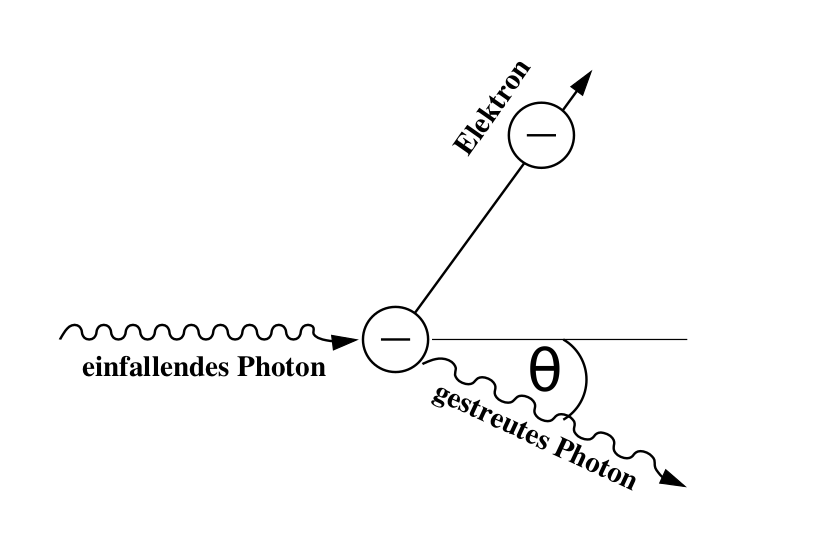
\includegraphics[scale=0.3]{content/comptoneffekt.png}
	\caption{Die Streuung eines Photons an einem Elektron.}
	\label{fig:StreuungPhoton}
\end{figure}
\noindent
Daher ist die Verschiebung dann minimal, wenn $\theta = 0 \si{\degree}$ und maximal, wenn $\theta = 180 \si{\degree}$ ist.
Hierbei wird der Term $\lambda_c = \frac{h}{m_e c}$ als Compton-Wellenlänge des Elektrons bezeichnet.

\subsection{Erzeugung der Röntgenstrahlung}
\label{sec:röntgenstr}
Um den Compton-Effekt beobachten zu können, muss zuerst Röntgenstrahlung erzeugt werden. Dafür werden in einer evakuierten Röhre aus einer Glühkathode Elektronen auf eine Anode zu emittiert.
Hierbei entsteht Röntgenstrahlung durch das Bremsspektrum und durch die charakteristische Röntgenstrahlung des verwendeten Materials der Anode.
\subsubsection{Das Bremsspektrum}
Wenn das Elektron in das Coulombfeld eines Atoms der Anode gelangt, wird es abgebremst und verliert Energie. Dabei wird ein Röntgenquant ausgesand. Dieses besitzt genau die Energie, die das Elektron durch das
Abbremsen verliert. Das Elektron kann hierbei nur einen Teil oder auch seine ganze Energie verlieren. So ergibt sich ein kontinuierliches Bremsspektrum.
\subsubsection{Das charakteristische Spektrum}
Das charakteristische Spektrum entsteht durch Ionisation der Anode. Durch die Ionisation kann ein Elektron aus einer höherenergetischen Schale Energie durch Abgabe eines Röntgenquants verlieren und in eine
niedriegere Schale fallen. Das Röntgenquant besitzt dann eine Energie, die gleich dem Energieunterschied der Schalen des Atoms ist. Daher ist das charakteristische Spektrum nicht kontinuierlich, sondern weist
scharfe Linien auf. Diese Linien sind charakteristisch für das Material der Anode.

\subsection{Die Bestimmung der Compton-Wellenlänge}
\label{sec:comptonwellenlänge}
Um die Compton-Wellenlänge zu bestimmen, wird verwendet, dass Aluminium Röntgenstrahlung sowohl transmittiert als auch absorbiert.
\subsubsection{Transmission der Röntgenstrahlung}
Zwischen der Transmission eines Stoffes und der Wellenlänge des einfallenden
Teilchens existiert ein Zusammenhang: je größer die Wellenlänge wird, desto weniger wird transmittiert. Aufgrund dieser Tatsache wird ein Teilchen mit durch den Compton-Effekt verschobene Wellenlänge weniger
transmittiert als eines vor Streuung an einem Elektron.

\subsubsection{Absorption der Röntgenstrahlung}
Das Delamber´sche Gesetz beschreibt die Intensität nach Absorption an einem Material der Dicke $d$:
\begin{equation}
	I = I_0 e^{- \mu d}.
	\label{eqn:intensitätabsorp}
\end{equation}
Hierbei ist $\mu$ der Absorptionskoeffizient. Dieser setzt sich wie folgt zusammen:
\begin{equation*}
	\mu = \mu_{Paar} + \mu_{Photo} + \mu_{Compton}
\end{equation*}
wobei $\mu_{Paar}$ den Absorptionskoeffizienten der Paarbildung, $\mu_{Photo}$ den des Photoeffektes und $\mu_{Compton}$ den des Comptoneffektes bezeichnet.

\subsection{Die Wellenlänge der Röntgenstrahlung}
Die Energie und die Wellenlänge eines Photons haben die Relation \eqref{eqn:E=hc/lambda}. Daher lässt sich Energie über Wellenlänge eines Photons bei Beugung an einem Kristallgitter mithilfe der
Bragg´schen Reflexion bestimmen. Wenn die Röntgenstrahlung auf das Gitter eines Kristalls fällt, werden die Photonen gebeugt und interferieren nach der Bragg´schen Bedingung:
\begin{equation}
	2 d \sin \alpha = n \lambda.
	\label{eqn:bragg}
\end{equation}
Hierbei bezeichet $d$ die Gitterkonstante des Kristallgitters, $\alpha$ der einfallende Winkel, $\lambda$ die gebeugte Wellenlänge des Photons und $n$ die Beugungsordnung.
